\documentclass[15pt,letterpaper]{article}

\PassOptionsToPackage{hyphens}{url}

\usepackage{setspace}
\doublespacing
\usepackage[]{natbib}
\bibliographystyle{apalike}
% \bibliographystyle{plainnat}

% === MARGINS ===
\addtolength{\hoffset}{-0.75in} 
\addtolength{\voffset}{-1.25in}
\addtolength{\textwidth}{1.5in} 
\addtolength{\textheight}{2.25in}

% == ENVS ==
\newenvironment{tightcenter}{%
  \setlength\topsep{0pt}
  \setlength\parskip{0pt}
  \begin{center}
}{
  \end{center}
}

% == PACKS ==
\usepackage{color,soul}
\usepackage{graphicx} % to use pngs in tex (include graphix)
\usepackage{calc} % To scale \pagewidth with \real{float}
\usepackage{pgfplots} % To draw histogram

\pgfplotsset{
  compat=1.17, 
colormap/viridis
} % request specific version of pgfplots

\usepackage{calc} % to use \real for text -> numeric
\usepackage{pgf} % to store numeric variables
\usepackage{subcaption} % to place two figures horizontally
\usepackage{caption} % to refer subfigure
\renewcommand{\thesubfigure}{(\alph{subfigure})}
\captionsetup[sub]{labelformat=simple}
\captionsetup[table]{font={stretch=1.2}}  % adjust line space in captions of TABLE and FIGURES
\captionsetup[figure]{font={stretch=1.2}}  


\usepackage{tikz}
\usetikzlibrary{automata,positioning}
\usetikzlibrary{arrows.meta, positioning, automata}
\usetikzlibrary{spy}
\usetikzlibrary{shadows}
\usetikzlibrary{arrows,positioning,shapes.geometric} % for dnn flowchart


\tikzset{
  font={\fontsize{10pt}{0}\selectfont}}
\usepackage{forest}
\tikzset{
  Decision/.style = {%
    draw,
    line width=1.4pt
  },
  Lottery/.style = {%
    draw,
    line width=1.4pt
  },
  Outcome/.style = {%
    circle,
    minimum width=3pt,
    fill,
    inner sep=0pt
  }
}
\usepackage{csquotes}
\usepackage{lipsum}
\usetikzlibrary{arrows.meta,automata,positioning} % to draw directed-weighted-graph


\usepackage{amsmath, amssymb, latexsym} % NN
\usepackage{tikz}% NN
\usetikzlibrary{decorations.pathreplacing}% NN
\usetikzlibrary{fadings}% NN


\usepackage{xltabular}
\usepackage{booktabs}

\usepackage[breakable, skins]{tcolorbox} % to add factual asepct inside a frame

\usepackage[title]{appendix}

%to prevent page and footnotes swalloen by the table


% == Checkmarks == 
\usepackage{bbding}
\usepackage{pifont}
\usepackage{wasysym}
\usepackage{amssymb}
% ================

% == BIBS ==
% \usepackage{natbib}

\usepackage{diagbox}

\usepackage[bottom]{footmisc}

\usepackage[
  hidelinks,
  pdftex, 
  bookmarksopen=true, 
  bookmarksnumbered=true,
  pdfstartview=FitH, 
  breaklinks=true, 
  urlbordercolor={0 1 0}, 
  citebordercolor={0 0 1}]
  {hyperref}

\usepackage[ruled,vlined,linesnumbered]{algorithm2e}
\SetKwFor{For}{for (}{) $\lbrace$}{$\rbrace$}

%%% Coloring the comment as blue
\newcommand\mycommfont[1]{\footnotesize\ttfamily\textcolor{blue}{#1}}
\SetCommentSty{mycommfont}

\SetKwInput{KwInput}{Input}                % Set the Input
\SetKwInput{KwOutput}{Output}   
\usepackage{algpseudocode}% http://ctan.org/pkg/algorithmicx
\usepackage{varwidth}% http://ctan.org/pkg/varwidth


\usepackage{titlesec}

\setcounter{secnumdepth}{4}

\titleformat{\paragraph}
{\normalfont\normalsize\bfseries}{\theparagraph}{1em}{}
\titlespacing*{\paragraph}
{0pt}{3.25ex plus 1ex minus .2ex}{1.5ex plus .2ex}


% == SPACES == 

% == CMMDS ==
\newcommand{\tit}{
\Large \bf
Analyzing the Treatment Effect of Committee Assignment on Stock Trading Patterns of Congressmen using Graph Neural Networks and Meta-Learners
}
\newcommand\spacingset[1]{\renewcommand{\baselinestretch}
{#1}\small\normalsize}

% To draw embedding layer
\newcommand*{\xMin}{0}%
\newcommand*{\xMax}{6}%
\newcommand*{\yMin}{0}%
\newcommand*{\yMax}{9}%
% To draw conv output
\newcommand*{\xMinOut}{10}%
\newcommand*{\xMaxOut}{11}%
\newcommand*{\yMinOut}{1}%
\newcommand*{\yMaxOut}{8}%


% == VARS == 
\pgfmathsetmacro{\heatmap}{1}

\makeatletter
\setlength{\@fptop}{0pt}
\makeatother

% == START (PageCounter, Mode)
\begin{document}

\spacingset{1.25}

\setcounter{page}{0}
\vspace{-.1in}

% == TITLE (includes DraftDate)
{\title{
    \tit
  }
  \author{
    Suyeol Yun
  \thanks{PhD Student, Department of Political Science, MIT. Email: \href{mailto:syyun@mit.edu}{syyun@mit.edu}\\
  % **The reproducible code and data can be found at the following link: \href{https://github.com/syyunn/efd}{https://github.com/syyunn/efd}.
  }
  }
  \maketitle
}

\thispagestyle{empty}
\vspace{-.1in}

\begin{abstract}
  This paper explores the relationship between congressional knowledge and stock trading patterns of members of Congress. While previous literature on this topic has only focused on excess returns, the ultimate goal of this research is to determine whether members of Congress use their privileged information to inform their trading behavior. The paper addresses a gap in the literature by performing a causal inference analysis to determine how committee assignment affects a member's trading behavior, and captures the congressional knowledge in the form of a social graph that includes committee assignments, bills, companies, and their interactions. A methodological challenge arises in transforming the graph-structured data into numerical representation for estimation of causal effects. The paper leverages the Graph Neural Network to generate a numerical representation and metalearners to effectively estimate the conditional average treatment effect. The research makes two significant contributions by identifying the effects of committee assignment on members' trading patterns and showcasing a novel method for estimating CATE using graph-structured data. 
  Overall, this paper provides valuable insights into the relationship between congressional knowledge and stock trading behavior and introduces a novel approach to performing causal inference on graph-structured data. 
\end{abstract}
\clearpage

% == INTRO ==
\section{Introduction}
\spacingset{2} % gives a slightly more margin between abstract and introduction
The investment behavior of congressmen has always been a topic of interest for researchers as it raises concerns about conflicts of interest \citep{TAHOUN201486}, insider trading \citep{Kim2012TheLT}, and abuse of power. Members of Congress have access to privileged and confidential information, such as pending legislation, government contracts, and upcoming regulations. 
If members of Congress use this information to make investments, it can be seen as unfair and unethical as they have an advantage over other market participants who do not have access to this information. 
Furthermore, people elect their representatives to Congress as delegates of their constituency to serve the public interest \citep{rep-del}, and not to enrich themselves personally. 
If members of Congress use their positions to gain financial benefits, it can be seen as a breach of public trust and may undermine the integrity of the democratic system.

Many studies have examined the investment behavior of congressmen, with the focus mainly on measuring their excess returns. Studies by \cite{zi11} and \cite{zi24} found that Senators and House representatives earn more than the market and enjoy excess returns, while a study by \cite{eg13} found that they do not. 
These studies aim to prove the existence of insider trading by measuring Congressmen's excess returns, which involves computing their average yearly return on investment. The approach assumes that, all else being equal, Congressmen's return should not exceed the market's average return, which is represented by index funds like the S\&P 500. 
However, this method is open to criticism because Congressmen may have a higher level of understanding of economics and financial markets. This may not necessarily be due to their privileged position, but rather because becoming a Congressman requires a higher level of education. As a result, their excess returns may have been affected by this factor.
Thus, measuring their excess returns alone does not prove whether they are using insider knowledge to make investments. 

Ultimately, the aims of research on this topic are to find evidence of conflicts of interest, where Congressmen prioritize their own interests over the public's interests, such as passing legislation that favors specific firms. Additionally, researchers aim to find an evidence that Congressmen engage in insider trading based on congressional knowledge that is not available to the public.


Unlike previous research that solely relies on the transaction data of Congressmen without specifying the exact source of congressional knowledge, 
this paper specifies the source of congressional knowledge that can affect congressional investment behavior.
For example,
interest groups are known to influence the legislative process by revealing their preferences and lobbying lawmakers \citep{smith}. 
They also provide policy information, political intelligence, and legislative assistance to policymakers \citep{hall_deardorff_2006}. 
Additionally, Congressmen are often assigned to multiple committees, where they oversee specific topics and organized interests. This allows them to expand their supportive coalitions and influence the content and fate of bills referred to the committee, which can be influenced by lobbyists. \citep{Hojnacki1998OrganizedIA}. 
As a result, members of Congress have access to detailed industry and firm-level information that can help them understand their policy preferences and the possible impact of certain legislation or political events on specific firms or industries.
All of these information can be regarded as congressional knowledge that can possibly affect their financial investment.
Therefore, to capture this congressional knowledge, the paper utilizes graph structured data\footnote{In network science, the terms ``graph'' and ``network'' are often used interchangeably to refer to a collection of nodes and edges, where the edges represent some sort of relationship or interaction between the nodes.}\footnote{Unlike the usual tabular data used in most political science research, graph structured data has the advantage of including the relationship between covariates in the form of connected edges between two nodes.} that includes the interaction between Congressmen, committees, firms, and bills in terms of their legislative and lobbying activities. 

To investigate whether congressmen use their knowledge gained through their position in Congress for personal stock trading, I am estimating the average effect that committee assignment has on the stock transaction patterns of congressmen. Specifically, I am examining how being assigned to a particular committee affects the similarity between a indutry-level bais of congressman's portfolio and the industry that the committee focuses on. 
This is measured by analyzing how firms that lobby on bills assigned to the committee are biased towards certain industries. Since committee assignments provide congressmen with important expertise in particular issue areas or industries \citep{Asher1974CommitteesAT}, if their transaction patterns become more similar after being assigned to a committee, it would suggest that they are using their congressional knowledge for personal investment purposes.
% The treatment is committee assignment, and the dependent variable is the similarity between Congressmen's stock transactions and their assigned committee where the treatment and dependent variables are both confounded by The independent variable is a graph that captures congressional knowledge based on the interaction between Congressmen, committees, firms, and bills in terms of their legislative and lobbying activities.

% To measure this similarity, the paper uses the cross-entropy between two distributions of NAICS codes, one from the Congressmen's stock transactions and the other from their assigned committee. 

% The stock transaction records of Congressmen contain firm-level information, including the company's stock they bought or sold, and the industry-level classification in which they operate. In addition, each firm lobbies on specific bills, and those bills are assigned to a committee, allowing for the aggregation of this information to obtain the NAICS code distribution of the assigned committee. By measuring the similarity between these two distributions, the paper examines how committee assignment to a certain committee affects the similarity of Congressmen's stock transactions to their assigned committee.

To justify the use of such a measurement, I will introduce some preliminary analysis that shows the mechanism of how insider trading occurs with actual transaction data. Congressmen typically acquire industry-level information from committees and identify critical points when certain political events could affect stock prices. They then design an industry-level portfolio based on this understanding, make transactions, buying and selling stocks before and after the critical points. To identify such insider trading, I present a method to estimate the possible excess return at the (Senator, Ticker)\footnote{A stock ticker is a unique series of letters assigned to a particular security traded on a stock exchange. It is also known as a stock symbol or ticker symbol, and is used to identify publicly traded companies and their stocks. For example, the stock ticker symbol for Apple Inc. is AAPL.} level, whereas previous literature \citep{zi11,zi24,eg13} only focuses on the Senator level in general. Additionally, although the raw data is somewhat censored, where the total amount spent for each transaction is given by range (known as interval-censored data), I will show how to estimate the probability distribution of excess return using a simulative method.

In addition, it is necessary to control for the confounders to estimate the effect correctly. I assume that the graph-structured data, which includes interactions between firms, bills, committees, and congressmen, and their stock transactions includes all possible confounders that affect committee assignments and their impact on the dependent variable, which is the industry-level similarity between the committee and the congressmen's portfolio. However, in terms of methodology, the question remains about how to control graph-structured data to estimate the treatment effect. Unlike tabular data with numeric values in each item, graph-structured data is a discrete object and thus cannot be computed in typical models.
However, thanks to recent developments in representational learning and neural networks, a specific architecture of neural network (called a ``Graph Neural Network'') can learn a good numeric representation of each node by considering its connection with its neighboring nodes in the graph.

To determine what constitutes a ``good'' representation of graph-structured data, one can evaluate whether the representation performs the downstream task effectively, which in this case is estimating CATE. The Graph Neural Network learns a representation, denoted as $\phi(X)$, for a given graph-structured data $X$, and I use $\phi(X)$ to estimate the effect of committee assignments on the dependent variable. However, because $\phi(X)$ will be a highly non-interpretable covariate that encodes complex interactions included in the graph, I use meta-learners \citep{metalearner} to estimate CATE using $\phi(X)$. Meta-learners are a family of estimators that combine supervised learning, also known as ``base-learners'', in a specific way while allowing the base learners to take any form, including neural networks. In this case, I use the Treatment Agnostic Regression Network (TARNet) \citep{tarnet}, which extends T-learners \citep{tlearner}, which is a variant of meta-learners, with additional layers of neural networks that learn a shared representation of $\phi(X)$ for the treatment and control groups in a balanced way. By doing so, the neural network can effectively perform its regression task to estimate CATE, even though $\phi(X)$ is complex, while jointly learning the balanced representation of $\phi(X)$.

In conclusion, this paper provides CATE estimates for all congressmen appearing in the dataset and reports the distribution of these estimates, along with the mean value ATE for all possible committees. On a substantive level, if these estimates are positive and have low variance, it suggests that committee assignments causally affect the congressmen's decision to hold more similar portfolios based on their committee-specific knowledge, which provides evidence that congressional knowledge is not orthogonal to their investment behavior. 

Overall, this paper has two main contributions. First, in a substantive manner, it proves the existence of insider trading by explicitly specifying the source of congressional knowledge and its impact on congressional investment behavior. Second, in a methodological sense, it demonstrates how to estimate causal quantities using graph-structured data by explicitly leveraging representation learning via Graph Neural Network.
% Therefore, this paper proposes a model and learning scheme that combines a Graph Neural Network and meta-learners to learn CATE, conditioning on the output of the Graph Neural Network. In sum, this paper showcases a way to estimate CATE using graph-structured data as input. The Graph Neural Network generates a representation of a given graph-structured graph X, which is denoted as phi(X). The following meta-learner then estimates CATE by learning a regression function E[Y(1)-Y(0)|phi(X)].

% However, the common limitation of these studies is that they do not specify the exact source of congressional knowledge and how that knowledge influences their investment behavior.

% Although many studies have investigated the investment behavior of congressmen, there are still gaps in the literature. \cite{zi11} and \cite{zi24} found that Senators and House representatives beat the market and enjoy excess returns while \cite{eg13} found that they don't. 
% However, the common limitation of current work is that they don't specify the exact source of congressional knowledge and how that knowledge affects their behavior.

% The biggest problem in this line of research is about how to prove they ``do'' invest with which ``privileged knowledge''.
% The main issue in this area of research is how to prove that politicians are using their inside knowledge to make investments. Just because they make a lot of money from their investments doesn't necessarily mean they are using privileged information. However, many high-profile cases have linked this knowledge to their committee assignments, sponsoring of bills, or their home state and potential connections to local businesses. Therefore, future research should focus on developing a reliable method to track down the sources of this privileged knowledge that is more closely linked to investments that show abnormally high returns. This will help to identify which politicians are involved in unethical financial practices and how they are doing it.

\section{Preliminary Analysis}\label{prelim}


In my initial research, I analyzed the excess return for each transaction made by Senators with specific stocks, comparing the return on investment to the federal reserve rates. The results, shown in Figure \ref{fig:agg-ex-r}, suggest that Senators do not generally make significant excess returns from their trading, which is consistent with the findings of \cite{eg13}. However, I did find a few outliers who made substantial gains, some of which have been reported by journalists, while others have not been publicly exposed. An important finding from these outliers is that committee information seems to enable some Senators to enjoy unusually high returns from their trading. 
For instance, Senator Ron Wyden from Oregon traded three semiconductor industry stocks, namely AMAT, KLAC, and AVGO, and gained a significant excess return of 170\%, 115\%, and 70\%, respectively (refer to Figure \ref{fig:agg-ex-r}). What stands out is that he bought all three stocks on the same day, April 6, 2020, during a time when the market was falling due to concerns about the pandemic's impact on the economy. He then sold all three stocks on the same day, April 6, 2021, after President Biden proposed a \$50 billion boost to the US chips industry. It is reasonable to assume that Senator Ron Wyden, being the chair of the Senate finance committee, had prior knowledge of this issue before it was made public. This is because the Senate finance committee introduced the bill ``S.3933 - CHIPS for America Act'' after the announcement on June 10, 2020.

As another example, Senator Ron Wyden made a 38\% ROI from his investment in an American wine producing company (Constellation Brand, Inc. - Ticker: STZ) when the Trump administration imposed additional tariffs on wines imported from Europe.
Since the Senate finance committee has jurisdiction over trade, it is reasonable to assume that Senator Ron Wyden had prior knowledge of this issue before it was made public.

In addition, David Perdue, a former senator from Georgia, obtained an estimated excess return of 10\% from his investment in BWX Technologies Inc., a company that supplies nuclear components to the US Navy. What is notable is that he made consecutive purchases of the stock that turned into sales after he was named chairman of the Senate Armed Services Subcommittee on Seapower.

\begin{figure}[h]
  \centering
  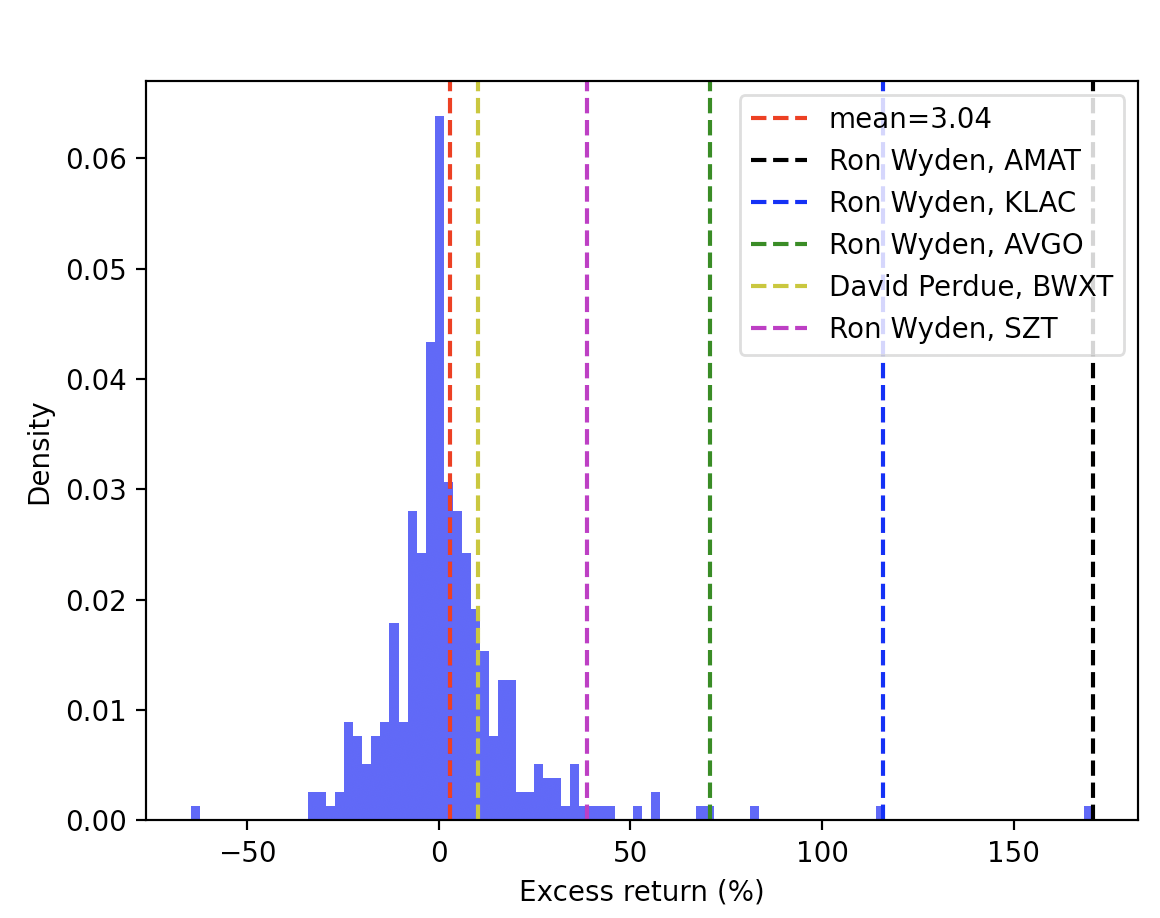
\includegraphics[width=1\textwidth]{imgs/ex-r/aggregate.png}
  \caption{Distribution of mean of each distribution of excess return for $333$ distinct pairs of (Senator, Ticker).}
  \label{fig:agg-ex-r}
\end{figure}

\begin{figure}[h]
  \centering
  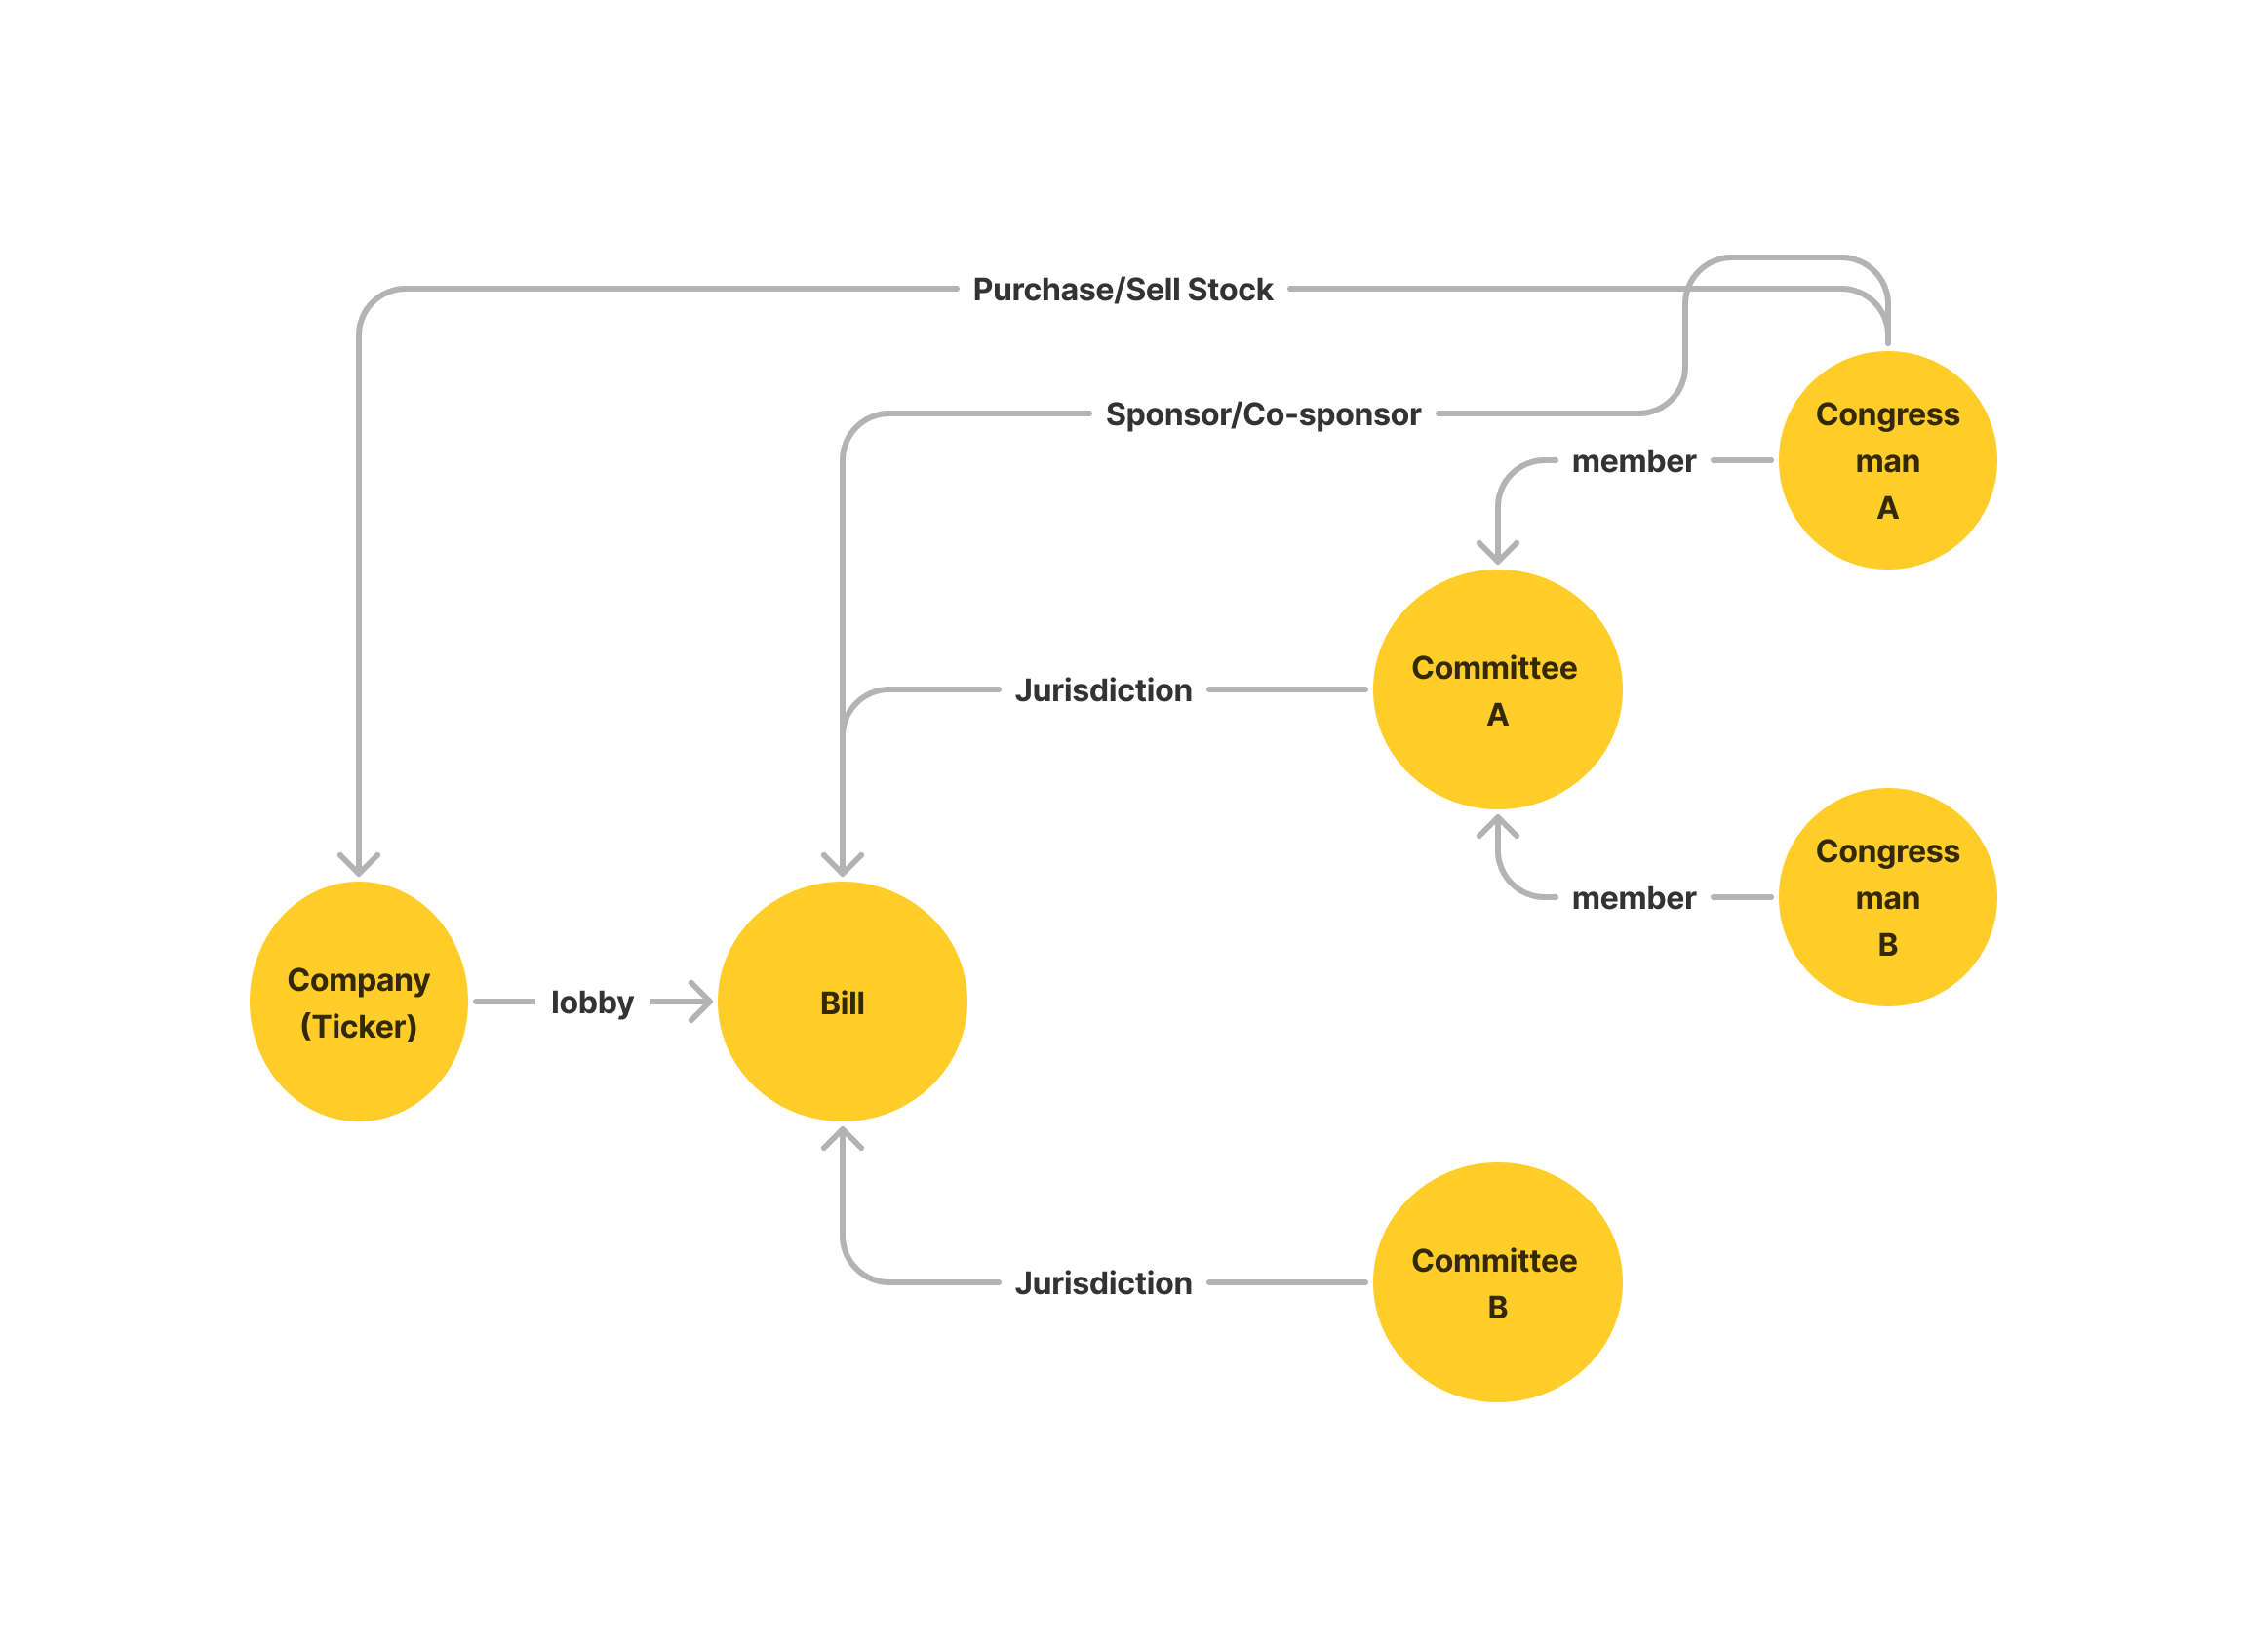
\includegraphics[width=1\textwidth]{imgs/cgd.png}
  \caption{Interaction graph between committees, bills, companies, and congressmen in congressional investment.}
  \label{fig:cbd}
\end{figure}


\section{Data and Methodology}
After analyzing the initial results, I have decided to investigate how committee membership impacts the trading behavior of Congressmen. Typically, each Congressmen is assigned to one or two committees, which are responsible for overseeing the legislation on a specific topic or bill. Companies that have a stake in the legislation have varying levels of interest and involvement, and this relationship is illustrated in Figure 2.

If the Lobbyview data is merged with my transaction data, it would be able to capture the 
 between bills, committees, companies, and Congressmen. Since these interactions can be represented as structured graph data, I plan to use a Graph Neural Network (GNN) for predictive analysis. The GNN will predict a Congressmen's investment in a specific stock using a graph network that includes information on bills, companies lobbying on those bills, committees with jurisdiction over those bills, and the Congressmen assigned to those committees.

A Graph Neural Network (GNN) is a type of neural network that can analyze graph-structured data. The main reason for using GNN in our research is because the data we are analyzing has a graph structure, representing different types of entities interacting with each other. Unlike traditional tabular data, graph data has a unique structure that requires a special type of model to process it. GNN can leverage the benefits of neural networks to encode complex patterns and dependencies in the graph data to effectively predict the quantity of interest, in our case the probability of stock trading of Congressmen. GNNs are also suitable for large-scale data analysis as the network involve a massive amount of data, with over 200,000 bills and 70,000 companies represented as nodes and their interactions as edges. GNNs can efficiently process such large-scale data by analyzing localized neighborhoods around each node.

Task-wise, I plan to use a Graph Neural Network (GNN) to perform a link prediction task. The input data will be a graph consisting of bills, companies, committees, and congressmen. The aim of the link prediction task is to predict which stock transactions are most likely to occur for a given congressman based on the interactions between these entities represented as a graph.

In addition, to make the GNN more interpretable, I will use a GNNExplainer \citep{gnne}, which will identify a subgraph that maximizes the mutual information with the GNN's prediction. 
Using the GNNExplainer will make the prediction task more interpretable, allowing us to understand how specific interactions between certain entities in the graph are likely to affect the prediction of stock transactions.
For example, for the prediction of Ron Wyden's semiconductor stock trading introduced in Section \ref{prelim}, I would expect GNNExplainer to provide a list of companies lobbied for CHIPS for America Act, like Samsung Electronics, Apple, Applied Materials, TSMC, QUALCOMM, Microsoft, Intel along with his committee memebership to the Senate Finance Committee as the ground of this prediction.
This information would help us understand why Ron Wyden made such trade.

\section{Conclusion}
The current literature lacks research on the specific information sources that lead to congressmen's stock transactions. Therefore, my research goal is to address this gap by identifying the source of information that instigated these transactions. To achieve this, I plan to merge the stock transaction data I collected with lobbyview data, which will allow me to capture the level of importance of committees to companies with lobbying activities.

Currently, I am merging this data and planning to use GNN for predictive analysis. However, before proceeding with deep learning using GNN, I am interested in knowing if there are other commonly used methods by political scientists to predict something with graph-structured data input. For my research, I will be using network data as input to predict each congressperson's stock trading activity.

Furthermore, I am seeking feedback on whether there are any ``causal-like'' estimands that can help achieve my research goal of identifying the primary source of information that congresspeople use. Currently, my approach using GNN with GNNEXplainer is purely predictive analysis and lacks a causal approach in a statistical sense. If there are any causal estimands that can help me achieve my goal, I would like to explore those avenues.

I have shared this research proposal with Insong, who agrees with my motivation and method. He is familiar with GNN as he has been working on a project using GNN with KAIST for over a year. I would like to know if this research direction would be persuasive for a political science paper in general.

Additionally, I am open to any straightforward advice to improve my research proposal. I am still in the early stages of my research, and I would appreciate any feedback to help me refine my approach. Please do not hesitate to share your thoughts.



\bibliography{biblo.bib}
\end{document}